% General Presentation:
%
%     Body text in a minimum 12 pt Times New Roman font
%     Single-spaced, with no more than 6 lines of type per inch
%     All margins set at a minimum of 3/4" (1.87 cm)
%     Font rules do not apply to text within tables and figures, but it must be clearly legible
%
% Your file must meet the following specifications:
%
%     PDF format (.pdf extension); unprotected
%     Maximum file size of 10 mb
%     8 ½" x 11" (216 mm x 279 mm) or A4 (210 mm x 297 mm)
%     Maximum 5 pages

%     References maximum 2 pages

% 2027 draft (C1), second pass. Structure and page budget: notes/proposal_outline.md.
% Title candidates (portal):
%   Prospective consequential life-cycle assessment: representing how markets and technologies
%     respond to decisions in energy and material transitions
%   Consequential life-cycle assessment for decisions in a world in transition: market and process responses

\documentclass[compact]{nserc} % use xelatex
\usepackage[]{csquotes}
\usepackage{booktabs}
\usepackage{tabularx}
\setlength{\textfloatsep}{8pt plus 2pt minus 2pt}
\setlength{\abovecaptionskip}{4pt}
\author{Guillaume Majeau-Bettez}
\addbibresource{references.bib} % cited entries only; see README for how to regenerate from Zotero
\addbibresource{/mnt/collection/zoterolibrary/zoteroFullLibrary_biblatex.bib}

\begin{document}
\noindent \textbf{Description of the Research Program}

\section{Context, research gap, and opportunity}

National decarbonization policies and international climate agreements are largely guided by energy system models (ESMs) and integrated assessment models (IAMs).\ci{Pauliuk2017} The IAM community has converged on a small set of internally consistent socioeconomic and mitigation pathways: the Shared Socioeconomic Pathways (SSPs) and Representative Concentration Pathways (RCPs).\ci{oneillNewScenarioFramework2014} Similarly, governments and industrial groups define roadmaps toward circular economy targets based on macro-scale material flow analyses (MFAs).\ci{aistRoadmapIronSteel2025,alonsoWorldMineralsOutlook,canadaplasticspactRoadmap2025Shared2021} These tools are designed to guide economy-wide decisions, such as national investment, taxation, and waste management policies. However, they lack the resolution to inform the everyday trade-offs made by industries and consumers. In other words, these macro-models have allowed for the exploration of useful global transition scenarios, but they are too coarse to offer specific guidance to the thousands of individual decisions that contribute to their implementation.

These micro-scale decisions are instead increasingly guided by attributional life-cycle assessment (ALCA), which estimates the share of environmental impacts linked, directly or indirectly, to a product or function.\ci{Hellweg2014,hellwegLifecycleAssessmentGuide2023} Carbon footprints, environmental product declarations, and organizational LCAs are now broadly employed in product design, corporate reporting, and sustainable consumption guidance. Most such assessments are \emph{retrospective}, relying on past data, which limits their use for forward-looking decisions in a rapidly transitioning economy. Prospective-ALCA (p-ALCA) databases such as premise now incorporate macro-scenario data into their processes and market mixes,\ci{sacchiPRospectiveEnvironMentalImpact2022} bringing temporal consistency to the assessment of long-lived products and future investments.

Major inconsistencies persist, however, between micro-scale p-ALCAs and macro-scale transition models, as energy systems illustrate. If an industry operates in a region already supplied by clean electricity, its p-ALCA results will show a limited contribution of electricity consumption to its footprint, and therefore limited benefits in further improving its energy efficiency. Yet, energy system models often identify efficiency gains in these same industries as essential for freeing clean electricity capacity to decarbonize other sectors. What appears negligible in a static footprinting assessment can thus be critical in the dynamic transition context. These contradictions arise because p-ALCAs remain \emph{attributional}: limited to the value chains under study, they cannot capture the market-mediated, system-wide consequences that shape the transition.\ci{Heijungs2001,Majeau-Bettez2017attribCons} Material cycles show the same problem: a p-ALCA may recommend maximizing the recycled content of a product, while dynamic material-flow analyses (dyn-MFAs) reveal that limited in-use stocks will constrain recycling supply for years.\ci{Pauliuk2015TakingStock} Increasing recycled content in one product may simply divert scarce secondary material from another, yielding little overall benefit.% These inconsistencies arise because all ALCAs are fundamentally unconstrained, linear models;\ci{Heijungs2001} they do not capture material or resource limits that are central to macro-scale transition strategies.

Capturing such bottlenecks and market-mediated mechanisms has long been the aim of consequential LCA (CLCA), which quantifies the direct and indirect environmental \emph{consequences} of changes in production and consumption.\ci{Zamagni2012} In short, whereas ALCAs describe how impacts are distributed within the value chains of a given economy, CLCAs quantify how impacts change when the economy itself is perturbed by an individual decision.\ci{Ekvall2004}

Yet, though theorized in the early 2000s,\ci{Ekvall2004} CLCA remains a niche approach.\ci{bamberComparingSourcesAnalysis2020} It requires identifying which suppliers would respond to a change in demand for each product (marginal suppliers),\ci{Weidema2003} which is highly uncertain and context-dependent.\ci{Mathiesen2009} Guidelines provide rules for this identification, and consequential databases have attempted to apply them across the economy,\ci{Weidema2003,vandepaerIntegrationLongtermMarginal2019} but with heterogeneous assumptions and little internal consistency; extensions of these rules to transition scenarios are only recent.\ci{maesProspectiveConsequentialLife2023,provost-savardGuidelinesProspectiveConsequential2025} These rules rely on market trends and very limited empirical data, and practitioners often restrict their detailed modelling to a small part of the product system (the foreground), leading to inconsistencies with background databases representing the rest of the economy. Building CLCAs has thus proven costly, and their results, resting on simplifications whose errors are largely unknown, are often hard to interpret and viewed with skepticism. Finally, CLCAs are almost always defined against a single scenario, the \emph{status quo} over the lifetime of the decision,\ci{Steubing2016} an assumption ill-suited to investment and production decisions in a rapidly evolving economy.

We see a \textbf{strategic opportunity} to make prospective CLCA (p-CLCA) a systematic bridge between macro-scale models (ESMs, IAMs, MFAs) and micro-scale decisions, anchoring each analysis as a perturbation of representative scenarios so that LCA guidance aligns with transition pathways.


\section{Core challenges and objectives}

We address two core challenges of CLCA through a common strategy.

The first challenge (\textbf{Pillar I}) is to represent how markets respond to marginal changes in demand. Sophisticated economic models would ideally capture this, but cannot be run for the thousands of markets in a CLCA, which are instead represented by simplifying heuristics. The problem is that these heuristics are currently (a) not bound by a consistent narrative, (b) wildly different in their level of sophistication, without characterization of their associated errors, and (c) inferred from trends rather than from the mechanisms that drive capacity investment (e.g., the timing of demand relative to peak in electricity systems). Our objective (\textbf{SO-1}) is therefore a scenario-consistent framework for identifying marginal suppliers: the responses of all markets in an assessment are derived from the same base scenario, by perturbing a model or applying heuristics to its outputs, informed by these mechanisms, and the errors of each level of simplification are characterized.

The second challenge (\textbf{Pillar II}) is to represent how technological processes respond to design and operating decisions and to deployment context. Sophisticated engineering models would ideally capture this, but cannot be built for the thousands of processes in a CLCA, which are instead represented with little parametrization or, most often, as fixed black boxes. Prospective databases make these black boxes evolve along macro-scenarios by rescaling selected inputs and emissions,\ci{sacchiPRospectiveEnvironMentalImpact2022} which aligns them with the scenario but not necessarily with the physics of the process. Where detailed engineering models are used in LCA, they are rarely formatted for reuse in other studies or for connection with other process models. These simplifications and incompatibilities (a) prevent the assessment of design and operating decisions in CLCA and (b) obscure real differences between variants of a technology by location, context and age; identifying the right marginal supplier (Pillar~I) is of little use if all suppliers share the same recipe. They also (c) make LCA work inefficient, limiting our community's ability to collaborate on common models and adapt them to different contexts. Our objective (\textbf{SO-2}) is therefore twofold: an interoperability framework that holds process models of any sophistication and represents specific technologies as instances of broader, coherent \emph{process-model classes}, instantiated from the base scenario for their context and technology evolution (grid mix, feedstock availability, vintage, efficiency frontier) and from the decision under study for their design and operation; and an efficient workflow to populate these classes with reduced engineering models, from data-rich established processes to emerging technologies.

They translate into three research questions:
\begin{itemize}
	\item \textbf{RQ-I.} How can the response of markets to a decision be derived consistently, from models of different types or from market evidence, down to the local markets where decisions play out, and what errors do common shortcuts introduce?
	\item \textbf{RQ-II.} How can technologies be represented so that what their variants share is modelled once, while the consequences of differences in context, vintage, operation and maturity are captured; and how can such models be built and reduced efficiently?
	\item \textbf{Program-level question.} Under which conditions do these representation choices change the decisions supported by p-CLCA, in the cases studied?
\end{itemize}

In both pillars, our \textbf{common strategy} is to (a) mirror each conceptual framework in open-source software, to support a change in community practice: an integration framework for market responses, implemented as an open layer on existing tools (e.g., premise, Brightway) in Pillar~I, and a modelling framework for process-model classes, implemented as a new open digital infrastructure in Pillar~II; (b) resolve what macro-scenarios aggregate, broad regions and technology classes, by representing the high-resolution interactions needed in LCA as specific instances of broader markets or of more general classes of processes, all derived from the same base scenario; (c) accommodate simplifying assumptions consistently, to fit differing levels of data availability and resolution; and (d) test these simplifications against more sophisticated models or observations to characterize their uncertainties and biases. We pursue these through CLCA case studies with differing data availability for market and process causation, each evaluated under at least two contrasting SSP/RCP base scenarios, including a low-demand pathway.\ci{debortoliMoreRationalityInclusivity2025}

These specific objectives contribute to our \textbf{long-term goal}: a p-CLCA practice built on shared, open representations of markets and technologies, maintained and extended by the community, that provides useful, pragmatic and discriminating decision support for consumption, process design and operation in a world in transition. % Our strategic positionning is that this is achievable if we maximize the use (and reuse) of available data and models through a smart integration and a flexible, open modelling framework; consolidation of these models as disaggregations and perturbations of macro-scenarios; and a systematic, quantitative approach to simplifying assumptions in the representation of economic and engineering causal mechanisms.

%\textbf{Long-term goal.} Our long-term goal is a consequential LCA that can tell decision-makers how a specific choice of technology, design, operation or deployment changes environmental flows in a world in transition, and how far that answer can be trusted. This requires representations of markets and technologies that are general enough to cover the economy, specific enough to respond to the decisions and contexts that matter, consistent with transition scenarios, and tested so that their errors are known. Beyond this grant, we aim to contribute to an open, community-maintained ecosystem of such representations. We do not compete with economists or process engineers on their own models: we build reductions of these models suited to consequential LCA, connect them consistently, and measure what each simplification costs in terms of decisions.

\underline{Recent progress:} Our recent work provides the starting points. For market responses, we developed guidelines and a timing-shift method for deriving marginal suppliers from IAM scenarios,\ci{provost-savardGuidelinesProspectiveConsequential2025} calibrated the open-source ESM EnergyScope-Quebec, and integrated LCA metrics in ESM optimization.\ci{souttreMescalToolCoupling2025} For databases, we regionalized ecoinvent with trade data\ci{agezRegioinventRegionalizedVersion2026} and pushed forward its reconciliation with mass conservation.\ci{dewachterMassbalancedEcoinventLife2026} For material flows, we built SSP-consistent aluminium scenarios,\ci{pedneaultSectorspecificScenariosFuture2022} quantified metal bottlenecks along IAM energy-transition scenarios,\ci{bieuvilleMetalBottlenecksEnergy2025} and assembled site-level databases on Canadian metal production.\ci{pellanDatasetMetalrelatedProduction2025,pellanSiteSpecificLifeCycleAssessment2026} For processes, we developed highly parametrized models of composting and hydrothermal carbonization.\ci{ravoahangyParametrizationBiowasteComposting2026,tanguay-riouxCanHydrothermalCarbonization2026} A prototype infrastructure for process models (v0) is being implemented with software-development support from the Canada Foundation for Innovation (CFI).


%% Too much in the weeds to early?
%\underline{Market responses are inferred from trends rather than from the mechanisms that produce them.} How a market responds to a change in demand depends on its state (growing, in overcapacity, constrained by resources or scrap), on the size and timing of the change and, for electricity, on when demand occurs. Practice compresses this response into rules applied to market trends: in a growing market, the technologies whose production grows are assumed to supply additional demand.\ci{Weidema2003} Consequential databases apply such rules to projected growth, because running energy-system models consistently for every market is impractical.\ci{vandepaerIntegrationLongtermMarginal2019} Applied to IAM outputs, they give results that are highly sensitive to the time interval chosen and differ substantially between models.\ci{maesProspectiveConsequentialLife2023} Moreover, growth does not show a response to demand: a technology may grow because of mandates or falling costs that would occur regardless of the decision. Energy research derives long-run marginal emission factors from models of capacity expansion,\ci{hawkesLongrunMarginalCO22014,gagnonPlanningEvolutionElectric2022} and early work showed that such analyses and simple rules can point to different marginal technologies.\ci{Mathiesen2009} But this practice is largely limited to electricity, the errors of the rules LCA uses instead have not been measured systematically, and for materials, open models that can be perturbed are scarce.

%% \underline{Technology representations are either generic or built case by case.} A useful representation must capture what the variants of a technology share, so that models are efficient to build and reuse, and how they differ in context, vintage, operating conditions, feedstock and maturity, since consequential questions often turn on these differences: whether an idle old plant or a new one responds, how a process is designed or operated, what an emerging process will look like once deployed.\ci{Majeau-Bettez2021} LCA databases offer breadth without this specificity. Each dataset describes one technology in one setting, is often transferred to other regions with few changes, and rarely distinguishes vintages or operating conditions. Regionalized databases, including our own Regioinvent, adapt the electricity, heat, waste treatment and supply markets a process draws on to its country, not the technology itself.\ci{agezRegioinventRegionalizedVersion2026} Site-level data show what this hides: across Canadian mining sites producing the same product, our assessment found impacts differing by up to a factor of 13, and by up to a factor of 6 from the proxy datasets normally used.\ci{pellanSiteSpecificLifeCycleAssessment2026} Parametrized and engineering process models offer specificity without breadth: each is built for one study or sector, with its own conventions, and is rarely designed to connect to others.

%Finally, consequential databases describe a single, near-present economy,\ci{Steubing2016} and prospective databases are mostly attributional.\ci{maesProspectiveConsequentialLife2023} Since consequences depend on the state of the economy (a growing market or one in overcapacity, scarce or abundant scrap), each decision should be evaluated against several internally consistent base scenarios.

%\textbf{Short-term objectives and approach.} Six objectives over five years, each carried by one trainee (highly qualified personnel, HQP), are organized in two pillars (Figure 1). Pillar I (market consequences) asks \emph{which units operate}: which suppliers respond to a decision, when, and where. Pillar II (process consequences) asks \emph{how they operate}: how processes and their environmental flows respond to design, operation, context and maturity. Both pillars follow the same plan, from known to unknown (rows of Figure 1): a representation is first developed and evaluated against a more complete model, then confronted with observed or reported data, and only then extended to settings without a full reference, relying on the errors measured before. The research questions are:


\begin{figure}[t]
	\centering
	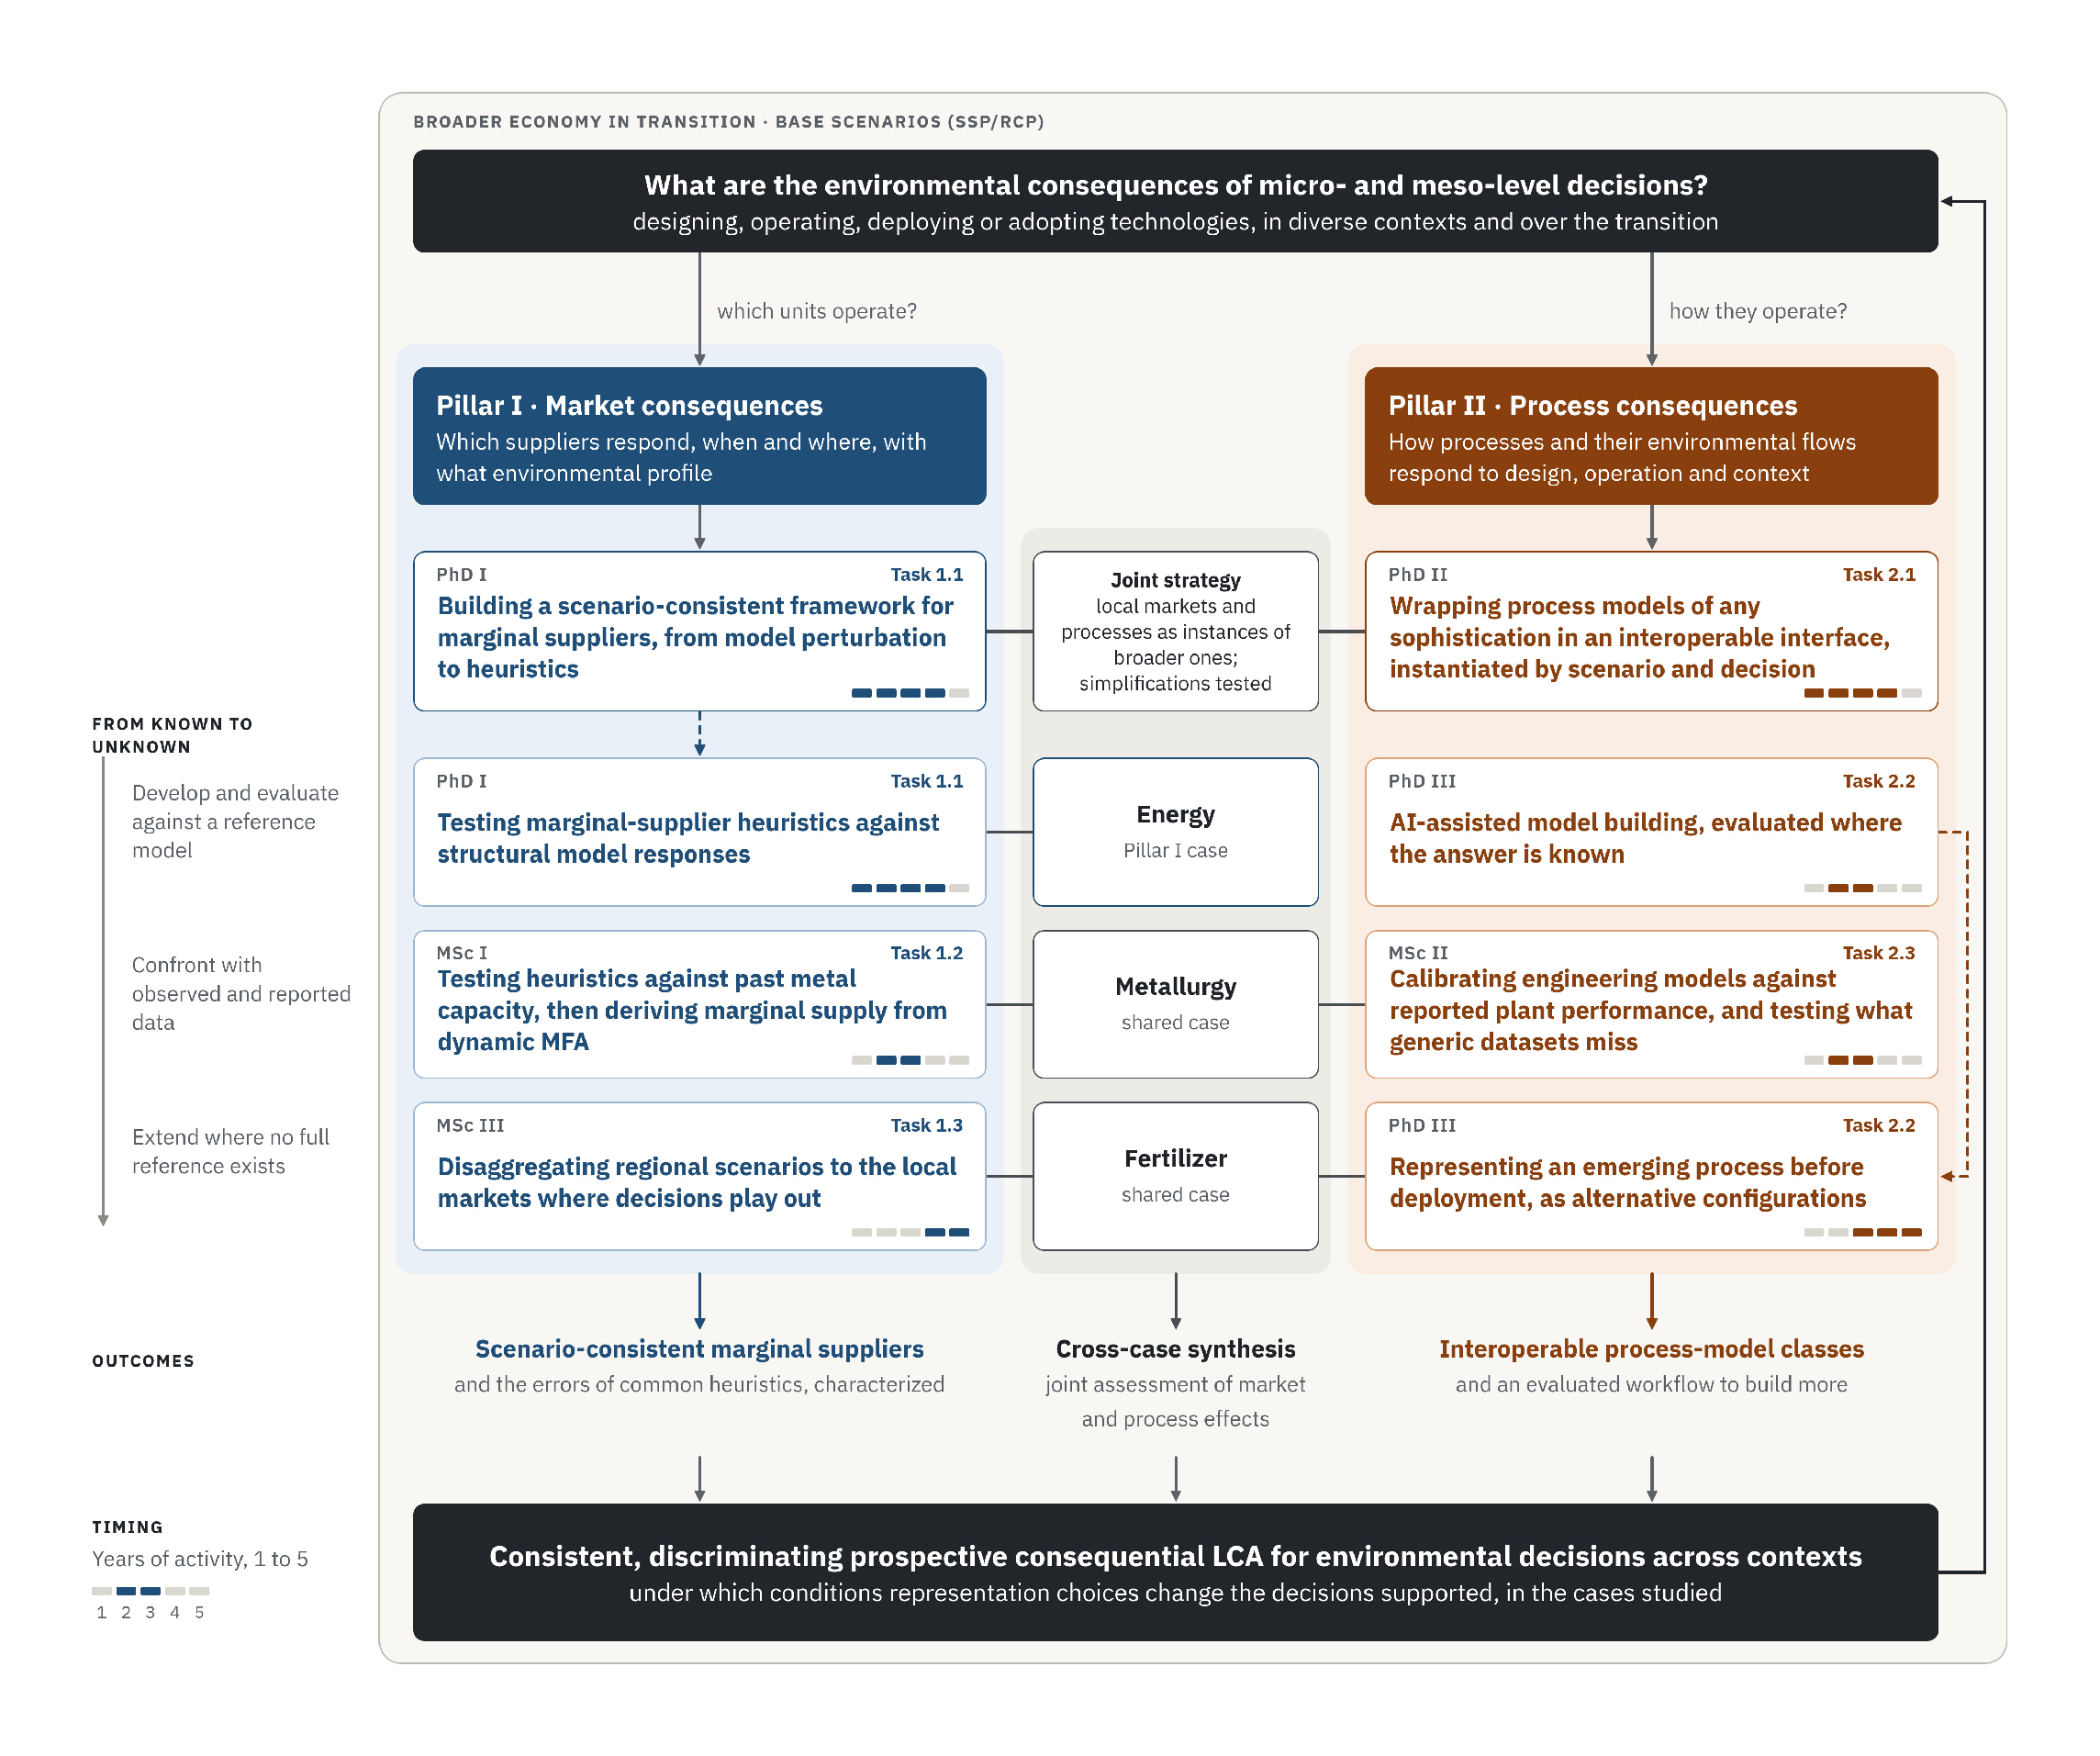
\includegraphics[width=0.86\textwidth]{figures/program_map.pdf}
	%\caption{Program map. Decisions enter both pillars. Each pillar has a core representation (top row), evaluated against references of decreasing strength (rows, from known to unknown). Cases (centre) and a shared protocol connect the pillars. HQP shown per objective.}
\end{figure}

%\section{Shared protocol: scenarios, perturbations and tests of validity}

%\textbf{Base scenarios.} Each decision is evaluated against several base scenarios: SSP/RCP pathways from published IAM ensembles,\ci{riahiSharedSocioeconomicPathways2017} completed for metals with stock-and-flow trajectories consistent with the same socioeconomic assumptions (O1.2). The set includes low-demand and sufficiency pathways, which mainstream scenario sets under-represent.\ci{debortoliMoreRationalityInclusivity2025,keysser2021degrowth} Scenarios set the market conditions of Pillar I, the boundary conditions of the regional energy model (import and carbon prices) and the context of process models in Pillar II (grid mix, feedstock availability). Results are reported with their robustness across scenarios.

%\textbf{Perturbations.} A decision is represented as a perturbation: a change in demand, design or operation, defined by its size, timing and profile and by whether suppliers can anticipate it, in the same way in every model. Changes in how a process is designed or operated (Pillar II) reach markets (Pillar I) through what they change in demand, such as a load profile or a co-product output.

%\textbf{Tests of validity.} The consequences of a decision cannot be observed directly: they are the difference between two futures, only one of which happens.\ci{oreskesVerificationValidationConfirmation1994} Validity is therefore tested in three ways. Internal consistency is checked in code on every model update: mass and energy balances, which our reconciliation of ecoinvent showed are far from guaranteed in current databases,\ci{dewachterMassbalancedEcoinventLife2026} supply equal to demand in each market, and production within capacity. Each simplified representation is compared with a more complete model where one can be run, and with observations where they exist (capacity actually built, plant statistics). Where neither exists, as for undeployed technologies, confidence rests on the errors measured in the first two settings. Both pillars use the same two success criteria: (i) agreement with the reference on the quantities that drive results, measured as the relative error on the impact intensity of the marginal supply mix (Pillar I) or of the main process flows (Pillar II); and (ii) preservation of decision rankings, measured as the rate of pairwise rank reversals across decision alternatives and impact categories. A small deviation that reverses a ranking counts as a failure. Tolerances are set for each case in the protocol, before results are known. The result is an error profile in the settings tested, not a universal threshold.

\section{Pillar I: market consequences}

%\textbf{Concept.} A market consequence is usually summarized by a marginal supplier or mix. We separate it into three questions that can each be tested: how much of a change in demand becomes a change in production, once prices and binding limits such as emission caps adjust; how much of that production comes from new rather than existing capacity, a share that changes over time; and which technologies and suppliers provide it. Current practice addresses mainly the third, assuming that extra demand is met in full by new capacity.\ci{vandepaerIntegrationLongtermMarginal2019} The output is a layer, built on existing open tools (pyam, premise, Brightway), that provides LCA databases with marginal supply mixes per market, documenting for each the scenario and the kind of evidence behind it. Artificial intelligence (AI) serves as a coding aid: it reduces the effort of scripting large batches of model runs and of building audited pipelines for market data, with every value traced to its source.

%\textbf{Approach.} The framework of SO-1 derives the marginal suppliers of every market from the same base scenario, so that all market responses in an LCA follow one transition narrative. Base scenarios are published SSP/RCP pathways,\ci{riahiSharedSocioeconomicPathways2017} including low-demand ones,\ci{debortoliMoreRationalityInclusivity2025,keysser2021degrowth} completed for materials, where IAMs are thin, by trajectories consistent with the same socioeconomic drivers (Task~1.2). Given the state of each market in the scenario (growth or decline, unused capacity), short-term responses are drawn from unused capacity, and long-term responses from changes in the timing of the scenario's capacity additions and retirements, building on our timing-shift method.\ci{provost-savardGuidelinesProspectiveConsequential2025} Because no single method suits all markets, the framework accepts methods of increasing simplification, and records which one was used for each market: perturbation of a structural model where one exists, heuristics applied to published scenario outputs, and market evidence (installed capacity, utilization, announced projects) where neither exists. The tasks measure what each simplification costs on two criteria shared with Pillar~II: agreement with the reference on the impact intensity of the marginal supply, and preservation of the ranking of decision alternatives, with tolerances set for each case before results are known. Tasks~1.1 to~1.3 test the framework against a structural model, then against observations, then extend it where no full reference exists (rows of Figure~1). The framework is released as open software built on existing tools (pyam, premise, Brightway).

\textbf{Task 1.1. Marginal suppliers tested against structural energy models} \emph{(SO-1; PhD~I, years 1--4).} \emph{How large are the errors of CLCA marginal-supplier heuristics relative to the response of a structural model, and on what do they depend?} %
%
The thesis first develops the SO-1 framework as consistent open-source software that captures the response of macro-models to perturbations and benchmarks simplifying heuristics against it, yielding scenario-tagged marginal supply mixes with their assumptions recorded. As a first application, we will apply marginal perturbations in the energy sector, under contrasting base scenarios, to at least one global IAM (likely the open-source GCAM, and MESSAGE through ongoing collaboration) and to a provincial dynamic ESM (EnergyScope-Quebec). Each model's own response serves as the reference for that model, and the two types are chosen for the different response mechanisms they expose rather than for a direct comparison. We will identify how far the response consists of changes in the utilization of existing capacity (short-term effects), in other actors' demand (demand elasticity, captured by the IAMs), or in new capacity (long-term effects). Perturbations will also differ in their load profile (e.g., winter-peaking heating versus flat industrial demand), to test whether the timing of demand, and not only its annual volume, determines the capacity that responds; EnergyScope-Quebec's peak-hour resolution captures this mechanism, which global IAMs represent only coarsely.

Of course, it is not generally feasible to directly perturb macro-models within a CLCA, and we will compare the above results to different heuristics applied to the baseline of the same model, at different levels of data availability. For example, what errors are introduced by our representation of perturbations as shifting the timing of planned investments in the transition scenario, compared to a full model run? How do these compare with heuristics based on trends in installed capacity or in production volume?

\textbf{Task 1.2. Material markets: hindcast and constrained secondary supply} \emph{(SO-1; MSc~I, years 2--3).} \emph{Would heuristics have identified the metal production capacity actually built, and when does extra demand for recycled metal fall on primary production? }
%
Unlike energy systems, metal markets lack open economic models that can be readily perturbed, but their past capacity additions can be observed. Looking backward, we apply CLCA heuristics to the information available at each date between 2000 and 2020 and compare the suppliers they identify, by vintage, with the capacity actually built, using plant trackers and company filings. This provides a falsification test of CLCA heuristics and of their domain of applicability. Looking forward, we then perturb a stock-driven MFA model under two or three SSPs to estimate prospective marginal supply mixes. Of particular interest is a capacity driver specific to metals, secondary supply constrained by in-use stocks and alloy quality: how sorting rates and the avoidance of inter-alloy contamination, a circular-economy priority, shape the evolution of the marginal mix and p-CLCA results. Cases are iron and steel (with ArcelorMittal, a long-standing CIRAIG partner) and aluminium, building on our SSP-consistent dynamic MFA of aluminium alloys.\ci{pedneaultSectorspecificScenariosFuture2022} \emph{Outcome:} a historical falsification test of marginal-supplier heuristics, and scenario-consistent trajectories of secondary metal supply for the framework.

\textbf{Task 1.3. From scenario regions to local markets} \emph{(SO-1; MSc~III, years 4--5).} \emph{Does representing local markets as instances of the markets of scenario regions change the marginal suppliers enough to change decisions? }
%
 IAM scenarios describe large world regions and broad technology classes; a growing regional trend can hide declining local markets. We will first apply the framework of Task~1.1 to fertilizer (nitrogen and phosphorus) markets, as forecasted by global MFAs and IAMs (notably GLOBIOM), to derive the evolution of their marginal suppliers under contrasting scenarios, at their native regional resolution. In these markets, resource concentration (phosphate rock) and trade shape which supply capacity responds; the study builds on our collaboration with OCP, a CIRAIG partner. We will then test different disaggregation algorithms (going beyond \textcite{sferraDSCALEV01Opensource2026}) to derive the evolution of local marginal suppliers, including the Canadian market, leveraging both demand-side data (local land use, demographic trends) and supply-side data (mine and plant capacities, trade flows, national plans), and compare the resulting marginal suppliers and impacts with those obtained at the native regional resolution. \emph{Outcome:} a tested method to derive the evolution of local marginal suppliers from global scenarios, and an estimation of its sensitivity to disaggregation assumptions.

\section{Pillar II: process consequences} %TODO expand title

% \textbf{Approach.} Pillar~II represents technologies as \emph{process-model classes} (SO-2). A steel-plant class, for instance, can be instantiated for Québec or China, today or in 2050, for a given vintage and operating state. The class holds what the variants share: structure, physical relations and quality checks (mass, energy and elemental balances, validity ranges). Parameters, and alternative structures where configurations differ, hold what distinguishes them. Behind the same interface, a class can hold models of any sophistication, from a fixed inventory to a detailed engineering model, so that a study can start simple and refine where it matters. Classes connect through interfaces that carry the links through which design and operation decisions propagate (co-products, feedstock use, load profiles), and instances are exported to standard database formats (EcoSpold2, Brightway). Process-systems engineering already couples process models with LCA, mostly against a fixed attributional background;\ci{Azapagic1999} our contribution is interoperability across models and the representation of these consequential links. SO-3 concerns the efficient generation of the reduced models that populate the classes, from data-rich established processes (Task~3.1) to documented and then emerging ones (Task~3.2); as in Pillar~I, each is evaluated against a reference on major flows and on the preservation of decision rankings. The prototype infrastructure (v0) embodies provisional design choices that this program evaluates and revises.

\textbf{Task 2.1. An interoperability framework for process models} \emph{(SO-2; PhD~II, years 1--4).} \emph{What must a process-model interface expose for models of any sophistication to be exchanged and connected without loss of consistency, and how far do current databases and published models fall short of it? }
%
The thesis starts by assessing the sophistication and quality control of process parametrization in consequential ecoinvent, a centralized CLCA database: the share of processes with (a) 100\% yields, (b) mass or energy balances that fail to close,\ci{dewachterMassbalancedEcoinventLife2026} or (c) one technology identical across regions and vintages. Reduced engineering models published in LCA studies are assessed likewise, together with their openness and reusability. We hypothesize a genuine tradeoff between high sophistication and flexibility in individual studies and high reusability in centralized databases, and that a decentralized interoperability layer can substantially reduce it.

The thesis then develops a framework for the \emph{decentralized} publication of interoperable process classes that can hold reduced process models of any kind, generalizing the prototype (v0) infrastructure developed for the 2PURES CFI project on plastic circularity. Its core design wraps technology models of any complexity (fixed inventories, machine-learning surrogates such as XGBoost, phenomenological models) in a compatibility layer that (a) enforces tests of physical plausibility, (b) separates the parameters set by the base scenario (context, vintage, efficiency frontier) from those set by the decision under study (design, operation), so that instances are derived consistently from macro-scenarios, and (c) exposes the flows needed to connect instances within a p-CLCA system. A central question concerns co-products, a long-standing focus of our group.\ci{Majeau-Bettez2017attribCons,provost-savardSubstitutionModelingCan2024} When operating conditions change the yields and qualities of co-products (for instance, the hydrochar and process water of hydrothermal carbonization, used as fuel, soil amendment or biogas feedstock), the substitutions they induce change too, and the interface must let the consequential treatment follow the operating state.

We will test the infrastructure by packaging parametrized models from the literature, instantiating them for different geographies and vintages, and connecting the instances to one another and to a consequential database. Success is measured by the share of published models that can be wrapped without loss of functionality and pass the plausibility checks, the share of their instances that connect consistently within the consequential database, and the effort required compared with conventionally inventorying the same variants; we will also quantify the influence of this disaggregation on consequential scores.  \emph{Outcome:} a general-purpose interface for developing and packaging process models, with documented design principles, tested on published models and through Tasks~2.2 and~2.3.


%This will be followed by a global sensitivity analysis\ci{kaddouraGlobalSensitivityAnalysis2025} that ranks the processes according to the probability that their variants could change results. This bounds the scope and yields an open screening tool.
%The thesis starts with an automated diagnostic of the level of specificity and physical representation of technologies in a centralized CLCA database (consequential ecoinvent). It will yield both a global sensitivity analysis of its parametrization and an assessment of the coverage and quality of this parametrization: share of processes tha (a) have an assumed yield of 100\%, (b) are represented by a single technological description across geographies or vintages, (c) break mass balance when feedstock composition is known, etc.

%The thesis then evaluates the v0 interface on a test suite in which the same processes, represented at several levels of sophistication (from database datasets to our parametrized composting and hydrothermal carbonization models\ci{ravoahangyParametrizationBiowasteComposting2026,tanguay-riouxCanHydrothermalCarbonization2026}), are exchanged within consequential systems, measuring consistency (closed balances, units and context passed between classes), the effort to exchange or connect a model, and the effect on results.



\textbf{Task 2.2. An efficient workflow, from documented to emerging processes} \emph{(SO-2; PhD~III, years 2--5).} \emph{Can a human-in-the-loop workflow build functional reduced models from publicly accessible material with much less effort, and with what errors? }%
%
Task~2.1 rests on the assumption that, in the long run, it is more efficient to invest in one common, quality-controlled technology model instantiated for different contexts than to inventory each geographical and vintage variant separately. In the short term, however, developing reduced engineering models remains a major investment. 
We investigate to what extent data collection, process modelling and coding can be automated with generative artificial intelligence (gen-AI) while keeping the resulting code documented and transparent, in a human-in-the-loop workflow: gen-AI drafts model code from first principles and published material, people review it, every parameter is traced to a cited source, and the built-in quality controls of Task~2.1 run as ordinary code. In years 2--3, the workflow is evaluated against reference models (our composting, biomethanization and hydrothermal carbonization models, and at least one model with little public documentation, to bound the advantage of well-documented processes), comparing structure, balance closure, outputs and effort. In years 3--4, it addresses a major uncertainty of low-maturity processes, the flowsheet itself, by assembling alternative configurations from reusable unit-operation modules and design heuristics,\ci{douglasHierarchicalDecisionProcedure1985} with maturity expressed through physical parameters (yields, specific energy) rather than generic learning rates, after checking that it recovers the configuration of a known process. In years 4--5, it is applied to plasma nitrogen fixation as a potential alternative to both fungicides and Haber-Bosch fertilizers, building on ongoing <+PLANET research+>; its alternative configurations are evaluated under the electricity and fertilizer-demand contexts of the base scenarios (Tasks~1.1 and~1.3). \emph{Outcome:} an evaluated workflow with its error profile, and a configuration-resolved model of an emerging process.

\textbf{Task 2.3. Reduced models of established, data-rich processes: metallurgy} \emph{(SO-2; MSc~II, years 2--3).} \emph{How far do engineering models of an established process deviate from reported plant performance, and does a calibrated, vintage-resolved model change consequential results relative to generic datasets?} %
%
First-principles reduced models can quickly grow a consistent base of reusable process models and explore novel technologies (Task~2.2), but may miss real-world performance; Task~2.3 tests them against well-documented plant data. It will develop a steel class resolved by vintage for one or two routes (blast furnace--basic oxygen furnace; direct reduction--electric arc furnace with natural gas, then hydrogen) from published engineering relations. In partnership with ArcelorMittal, it then adds a calibration step to the workflow of Task~2.2: estimating, from plant and sector statistics, the inefficiencies that design models leave out (part load, start-ups, losses). The calibrated class is then instantiated along scenario trajectories (scrap availability from Task~1.2, vintage structure of installed capacity), and the efficiency improvements that IAM scenarios assume for the sector are checked against its physical limits. The calibrated class is compared with its uncalibrated version and with ecoinvent datasets, for internal consistency and effect on consequential results. \emph{Outcome:} a calibrated, reusable steel class, a measure of what generic datasets miss, and a physical consistency check of scenario assumptions for steel.

\section{Integration, plan and risks}

Integration does not wait for the end of the program. A cumulative table of case results, shared across pillars, is set up in year 1 and maintained by PhD I and PhD II. Energy is a Pillar I case; metallurgy and nitrogen are shared by both pillars (centre of Figure~1). On metallurgy (years 2--3, with ArcelorMittal), Tasks~1.2 and~2.3 test whether distinguishing idle, often old, capacity from new capacity close to best available technology changes which supplier responds and with what flows. On nitrogen (years 4--5), Tasks~1.1, 1.3 and~2.2 ask which matters more for an emerging process: uncertainty about its deployed configuration, or about the market responses it triggers (electricity demanded, fertilizer displaced).

%\par\smallskip\noindent{\small
%\begin{tabularx}{\textwidth}{@{}p{0.40\textwidth}llX@{}}
%\toprule
%Objective & HQP & Years & Key milestone (year)\\
%\midrule
%O1.1 Market responses in perturbable models & PhD I & 1--4 & EnergyScope Québec perturbation study (2)\\
%O1.2 Metallurgy: hindcast and trajectories & MSc I & 2--3 & Steel hindcast of marginal-supplier rules (3)\\
%O1.3 From regional scenarios to local markets & MSc III & 4--5 & Country-level marginal ammonia supply (5)\\
%O2.1 Representation of process-model classes & PhD II & 1--4 & Database diagnostic, screening tool (2)\\
%O2.2 AI-assisted construction and anticipation & PhD III & 2--5 & Workflow evaluated on known processes (3)\\
%O2.3 Metallurgy class, benchmarked & MSc II & 2--3 & Steel class compared with ecoinvent (3)\\
%\bottomrule
%\end{tabularx}}\par\smallskip

\textbf{Risks and fallbacks.} Each task yields publishable results on its own. If global IAMs prove too costly to operate, Task~1.1 rests on EnergyScope Québec and published scenario outputs. Should data or time become limiting, Task~1.2 restricts its scope to a single metal, steel unless its data are inaccessible, in which case Task~2.3 also switches to aluminium. If the AI-assisted workflow underperforms, its measured error profile is itself a result, and classes are built conventionally. If plasma results are too immature, the configuration method is applied to another emerging process studied by our group.

\section{Open infrastructure, partners, equity and significance}

\textbf{Open infrastructure and its maintenance.} The Pillar~II infrastructure is a decentralized open protocol, not a new central database. Class interfaces, quality checks and reference implementations are open (versioned releases, continuous integration); parameter sets and instances may be held under different licences (licensed databases, confidential company data exported as aggregated inventories), provided they pass the same checks. Results that depend on ecoinvent are regenerated by licensed users, and outputs feed tools that are already maintained (premise, Brightway, Regioinvent, mescal). Long-term maintenance of the core is supported through the CIRAIG (International Reference Centre for Life Cycle Assessment and Sustainable Transition), whose industrial research chairs have been funded continuously by partners for about 25 years.

\textbf{Partners.} ArcelorMittal, Hydro-Québec and Québec's Ministère de l'Économie, de l'Innovation et de l'Énergie are full CIRAIG partners, contributing funding, data and engagement. In the metallurgy and energy cases, they help define the decision alternatives to compare, so that the ranking criterion is tested on decisions that matter in practice.

\textbf{Relevance for equity and environmental justice.} Consequential LCA asks not only how large the consequences of a decision are, but where they fall: which mines, smelters or power plants respond, and therefore which communities bear the resulting burdens.\ci{holland2016electricvehicles,owen2023landconnected} Generic datasets, often derived from European or North American contexts, average this distribution away. Our research makes it visible at three levels: marginal suppliers resolved to local markets and, where data allow, to individual plants (Tasks~1.2 and~1.3);\ci{pellanDatasetMetalrelatedProduction2025} technology variants resolved by age and emission controls, since a minority of old, poorly controlled units concentrates pollution where these fleets operate;\ci{tong2018superpolluting} and process models recontextualized beyond the high-income regions that dominate LCA data. Results will be reported by region and compared with public spatial data on characteristics relevant in Canada (income, Indigenous lands, remote regions). These results can provide useful information for analyses of distributional justice; they do not address procedural justice, which would require community partnerships we do not claim.\ci{jenkins2016energyjustice}

\textbf{Subjective choices in our methods.} Several modelling choices in this program are not neutral, and we will treat them as explicit assumptions rather than technical defaults. (i) Base scenarios embed assumptions about growth and inequality; we include low-demand pathways, which mainstream scenario sets under-represent.\ci{debortoliMoreRationalityInclusivity2025,keysser2021degrowth} (ii) Marginal-supplier methods assume that markets respond through least-cost investment, which places new capacity where production is cheapest, a choice with fairness implications;\ci{pachauri2022fairness} the framework records the assumptions behind each market response. (iii) Engineering literature and AI models are skewed towards high-income regions,\ci{manvi2024llmgeobias} so the evaluation of Task~2.2 includes process instances outside high-income countries where reference data exist, and recontextualized instances carry data-quality flags so that they are not mistaken for local data. (iv) Time horizons and weighting sets can reverse rankings, and preferred weights differ between income groups,\ci{deschryver2013valuechoices,bayazitsubasi2024weighting} so rankings are reported under alternative value sets. Each case study records these choices in a shared assumptions register, reviewed with its trainees.

\textbf{Significance.} We do not aim to resolve every difficulty of CLCA, but the core limitation that has kept it marginal: its results rest on representations of markets and technologies that are inconsistent with one another and with transition pathways, and whose errors are unknown. Lacking a trusted alternative, decision-makers routinely answer consequential questions with attributional tools, which can mislead them.\ci{Ekvall2004} By deriving market responses and technology representations from the same macro-scale scenarios, this program aims to make p-CLCA consistent and aligned with transition pathways, and to characterize, in contrasting cases, what common simplifications cost. Crucially, it delivers this as a workflow and an open infrastructure that others can adopt and extend: market responses tied to declared scenarios, and process-model classes that the community can instantiate, refine and connect, rather than rebuilding inventories study by study. Its reach would therefore extend well beyond our own cases: if successful, it would change what the LCA community can offer, answering consequential questions with consequential tools, at the resolution of individual design, operation and deployment decisions. For Canadian decision-makers in metallurgy, fertilizer and electricity, it will provide a way to test whether such choices support the transition pathways they plan for. Its HQP will combine LCA, system models, process modelling and verified data pipelines.

\pagebreak
\setcounter{page}{1}
% Renew geography
\newgeometry{left=1.9cm, right=1.9cm, top=1.9cm, bottom=1.9cm, headheight=15pt}
\begingroup
\setlength\bibitemsep{0pt}
%\begin{multicols}{2}
\printbibliography
%\end{multicols}
\endgroup

\end{document}
